% \section{Le Projet}
% \subsection{Objet du document}

% Ce document a pour objectif le suivi du projet " Atelier logiciel - système de transmission "

% Vous trouverez dans ce document l'ensemble des itérations, les tests réalisés, et les modifications apportées tout au long du projet.

% \subsection{Cahier des charges}

% L'objectif consiste à transmettre un message d'un point d'entrée à un point de sortie, via un canal de transmission (ou de communication). Le message d'entrée est émis par une source d'entrée. Les messages considérés dans ce projet seront des suites de symboles binaires (0 ou 1) correspondant à des informations échantillonnées et quantifiées sur deux niveaux logiques. Le message de sortie sera - autant que faire se peut - semblable au message d'entrée. Ce dernier étant incapable de traverser le canal de propagation tel quel, on l'adaptera aux caractéristiques physiques du canal en le convertissant au moyen d'un transducteur en un " vecteur " adapté à la transmission, appelé signal.

% Ce dernier sera injecté dans le canal au moyen d'un émetteur. À l'autre extrémité du canal, il sera récupéré et traité par le récepteur et le transducteur de réception.

% Les principaux canaux de transmission rencontrés dans la nature sont : le canal Hertzien (espace libre), le canal guidé électrique (câble), le canal guidé Optique (fibre), le canal acoustique aérien et le canal acoustique sous-marin. Chaque canal de propagation devant être utilisé à une fréquence bien particulière, le message est transposé autour de cette fréquence par l'opération de modulation. En outre, le canal sera une source de bruit pour les signaux qu'il transporte. Les principales sources de bruit rencontrées en pratique sont : la dispersion de trajets, la dispersion chromatique, le bruit de détection (grenaille), le bruit thermique et le bruit d'amplification.

% Par la suite, chaque composant du système de transmission entre la source et la destination sera dénommé transmetteur.

% \begin{figure}[h]
%     \centering
%     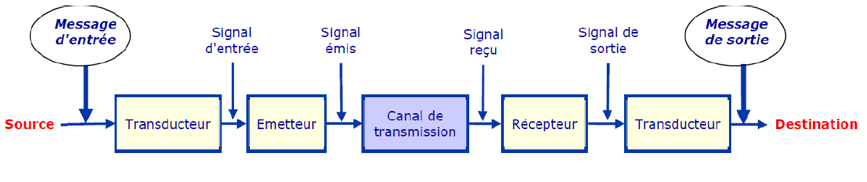
\includegraphics[width=1\textwidth]{image 1.png}
%     \caption{\label{fig:image1}Composants de la chaine de transmission.}
% \end{figure}
% \newpage
% \section{Iteration n°1}
% \subsection{Objectifs}

% L'objectif de cette première itération est avant tout de prendre en main la chaine de transmission.

% Pour cette itération, la chaine respectera les propriétés suivantes :

% La source émet une séquence booléenne soit fixée, soit aléatoire.
% Le transmetteur logique parfait se contente, à la réception d'un signal, de l'émettre tel quel vers les destinations qui lui sont connectées.
% La destination se contente de recevoir le signal du composant sur lequel elle est connectée.
% Des sondes logiques permettent de visualiser les signaux émis par la source et le transmetteur parfait.
% L'application principale calcule le taux d'erreur binaire (TEB) du système.

% Voici un schéma de la chaine :

% \begin{figure}[h]
%     \centering
%     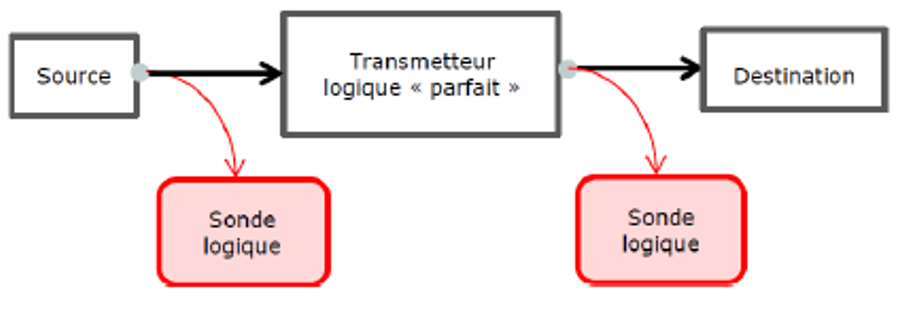
\includegraphics[width=1\textwidth]{image 2.png}
%     \caption{\label{fig:image2}Chaine de transmission itération 1.}
% \end{figure}

% \subsection{Actions réalisées}

% \subsubsection{Sources}

% Dans un premier temps, nous avons créé deux classes sources. Une source fixe, qui envoie toujours la même séquence de données. Puis une source aléatoire qui envoie une nouvelle séquence à chaque appel.

% \subsubsection{Transmetteur}

% Par la suite, nous avons créé un transmetteur parfait. Il joue le rôle du canal de propagation. Pour ce transmetteur parfait, le canal transmet exactement ce qu'il reçoit.

% \subsubsection{Destination}

% Enfin, nous avons créé une destination. Cette classe joue le rôle de récepteur dans la chaine de transmission.

% \subsection{Simulation}

% Voici la simulation avec une source fixe :
% \begin{figure}[h]
%     \centering
%     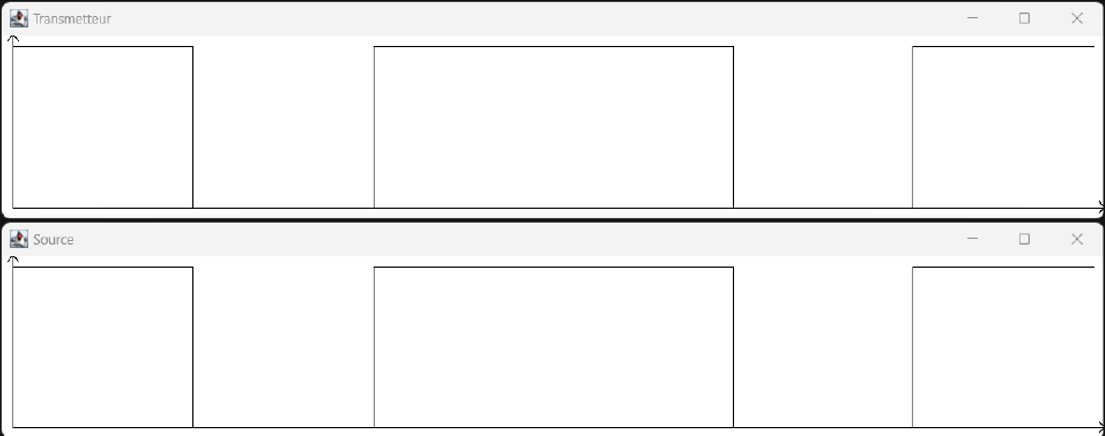
\includegraphics[width=1\textwidth]{image 3.png}
%     \caption{\label{fig:image3}Simulation source fixe source et transmetteur.}
% \end{figure}

% Voici la simulation avec une source aléatoire :
% \begin{figure}[h]
%     \centering
%     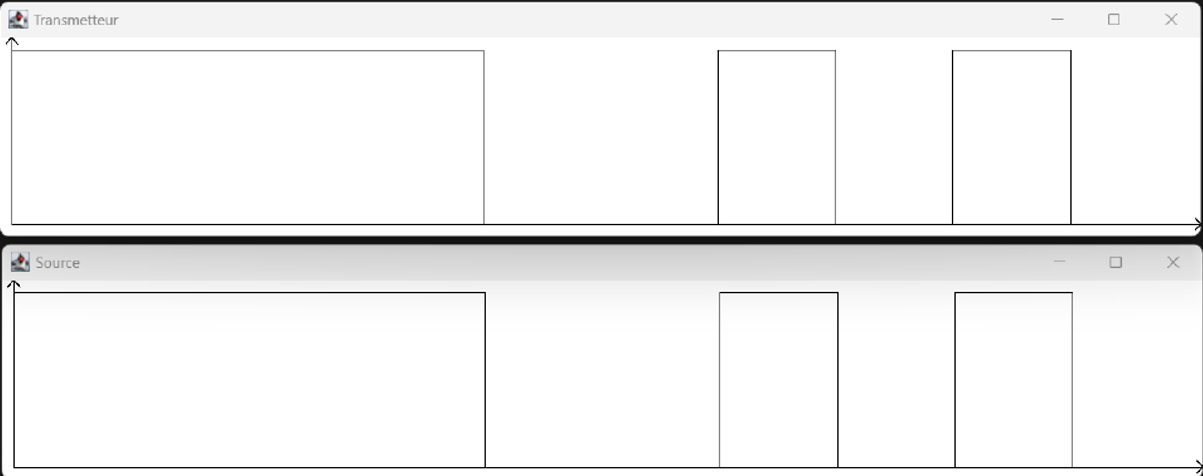
\includegraphics[width=1\textwidth]{image 4.png}
%     \caption{\label{fig:image4}Simulation source aléatoire source et transmetteur.}
% \end{figure}

% Nous observons que la sortie du transmetteur est purement identique à la source. C'est normal car il s'agit d'un canal parfait. Le TEB est donc de 0.

% \subsection{Conclusion}

% Pour conclure, notre chaine de transmission est fonctionnelle, nous sommes en mesure de choisir le type de source et observer la sortie du canal.

% Pour le moment, nous n'avons qu'un seul type de transmetteur et que deux types de sources. Par la suite, nous serons amenés à mettre en œuvre une chaine de transmission avec des signaux analogiques et des canaux de propagations non-parfaits.
% \newpage
\section{Etape 2}
\subsection{Objectif de l'itération}

Dans cette nouvelle itération, nous allons devoir coder des émetteurs et un récepteur afin de convertir le signal logique en un signal " analogique " NRZ (non-retour à zéro), RZ (retour à zéro) et NRZT. Le rôle du récepteur sera de convertir n'importe quel signal analogique en un signal logique. Pour se faire, nous allons donc devoir modifier notre code afin de répondre aux exigences.

\begin{figure}[h]
    \centering
    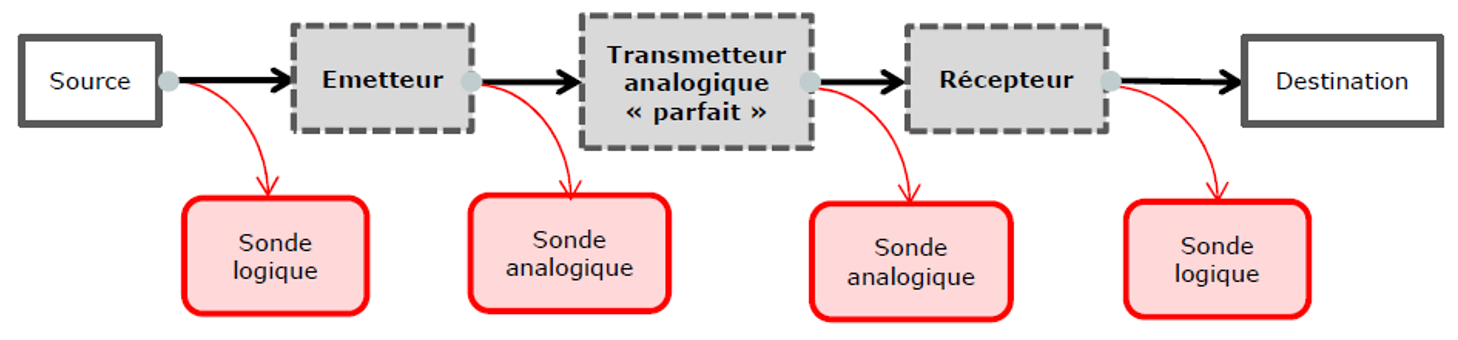
\includegraphics[width=1\textwidth]{image 5.png}
    \caption{\label{fig:image5}Chaine de transmission itération n°2.}
\end{figure}

Un signal RZ signifie que le signal sera à l'état haut lorsque des 1 logiques seront transmis et à l'état bas lorsqu'il s'agit de 0 logique pendant la première demi-période. Il y a un retour à 0 à la deuxième demi-période du symbole (figure de gauche). Cependant dans ce projet, nous partirons du principe que l'émission à Vmax ou Vmin se situe entre le 1er et le 3ème tiers de la période symbole (figure de droite).

\begin{figure}[h]
    \centering
    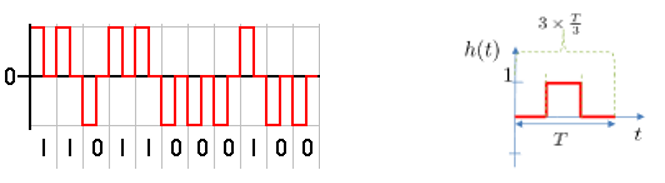
\includegraphics[width=1\textwidth]{image 6.png}
    \caption{\label{fig:image6}Schémas explicatifs signal RZ.}
\end{figure}

Un signal NRZ signifie que le signal sera à l'état haut lorsque des 1 logiques seront transmis et à l'état bas lorsqu'il s'agit de 0 logique. Contrairement au RZ, l'état est le même pendant toute la durée du temps symbole et d'utiliser deux fois moins de bande passante.

\begin{figure}[h]
    \centering
    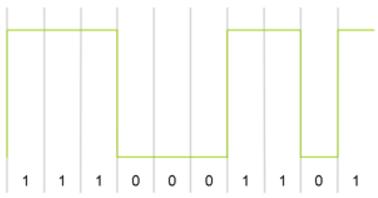
\includegraphics[width=0.5\textwidth]{image 7.png}
    \caption{\label{fig:image7}Schéma explicatif signal NRZ.}
\end{figure}

Un signal NRZT possède les mêmes propriétés qu'un signal NRZ. Cependant pour simuler le temps de montés des composants, chaque changement d'état sera représenté par une monté et descente progressive symbolisé sur 1/3 des périodes symboles.

\begin{figure}[h]
    \centering
    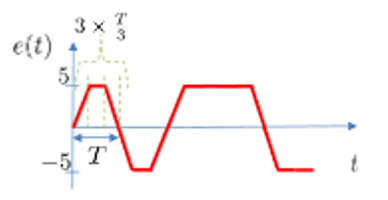
\includegraphics[width=0.5\textwidth]{image 8.png}
    \caption{\label{fig:image8}Schéma explicatif signal NRZT.}
\end{figure}

\subsection{Organisation}

Pour nous permettre de répondre aux demandes de l'itération (mise en place d'une transmission analogique), nous allons devoir créer deux nouveaux éléments par rapport au code de la première itération. Ces modifications devront nous aider à lancer le programme tout en prenant en compte les paramètres d'entrée que nous rentrerons dans le terminal.
Nous ne devrions plus avoir d'erreurs sur notre code et ne pas avoir d'erreurs sur les signaux émis et reçus. Pour vérifier cela, nous utiliserons le calcul du TEB et afficherons les graphiques permettant de comparer à vue d'œil les éventuelles erreurs et leur emplacement.
Avant de commencer à développer notre code nous avons utilisé l'application " Project " d'Office 365 afin de nous permettre de créer un diagramme de Gant. Ce diagramme nous permet de classer les actions à faire (par catégories, par acteurs, par priorité) et de mettre des échéances afin de respecter les délais. Vous trouverez ci-dessous un exemple de diagramme Gant que nous avons fait pour cette seconde itération :

\begin{figure}[h]
    \centering
    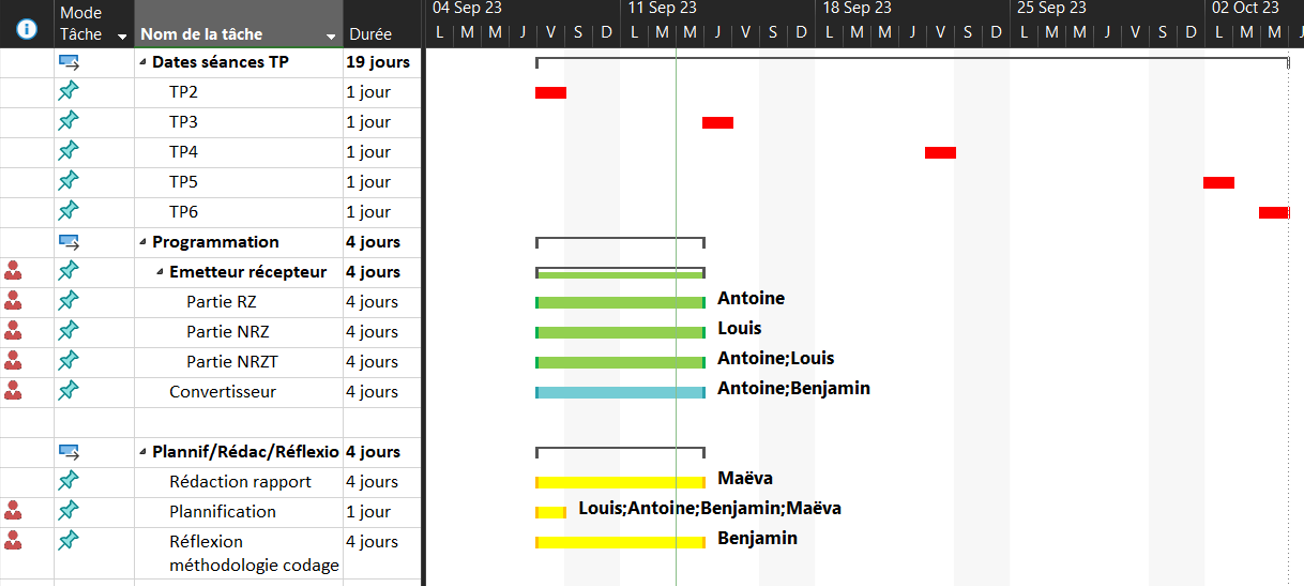
\includegraphics[width=1\textwidth]{image 9.png}
    \caption{\label{fig:image9}Diagramme de Gant itération 1.}
\end{figure}

Pour le développement de notre code, nous allons utiliser l'application Intellij Idea nous permettant de partager plus facilement les codes que nous déposons sur le projet que nous avons créé sur GitLab. La combinaison des 2 nous permet de modifier le code tous en même temps sans empiéter sur les modifications des-uns et des-autres. Intellij Idea nous permet également de créer des branches et de ne commit sur une interface graphique. Il est donc important de se répartir les tâches, ce que nous avons fait dans le diagramme de Gant.

\subsection{Procédures de développement}
\subsubsection{Emetteur}

L'émetteur à un rôle important. Il permet de convertir un signal logique en signal pseudo-analogique. Trois codages en ligne sont attendus pour ce projet. La logique qui repose sur ceux-ci sont la même. On prend le signal logique en entrée, puis en fonction de son état (0 ou 1), on le transforme en une série de flottant qui sera adapté au codage en ligne souhaité. Le nombre d'échantillonnage par symbole sera un paramètre à choisir lors des lancements de simulations (nommé nb\_samples par la suite) ainsi que l'amplitude maximum (Vmax) et minimum (Vmin).

\textbf{Emetteur NRZ :}

Il s'agit de l'émetteur le plus simple à coder. On prend le symbole logique en entrée et s'il s'agit d'un état à 1, alors on émet un nombre de flottant égale à nb\_samples ayant pour amplitude Vmax. Pour l'état à 0, on émet le même nombre de flottant mais ayant pour amplitude Vmin.

\begin{figure}[h]
    \centering
    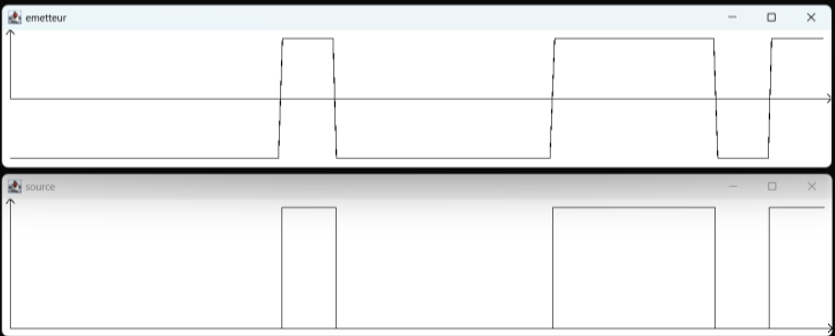
\includegraphics[width=1\textwidth]{image 10.png}
    \caption{\label{fig:image10}Sortie de la source et de l'émetteur NRZ.}
\end{figure}

Ci-dessus le graphique en sortie de la source et de l'émetteur NRZ. On retrouve bien une amplitude égale à Vmax pendant une durée symbole pour un état logique 1 et une amplitude égale à Vmin pendant une durée symbole pour un état logique à 0.

Emetteur RZ :

L'émetteur RZ est légèrement plus compliqué que le signal NRZ. La construction d'un symbole se passe en trois étapes.

\begin{itemize}
    \item Sur le premier tiers $(\frac{nb\_samples}{3})$, les flottants ont pour amplitude 0.
    \item Sur le deuxième tiers $(]\frac{nb\_samples}{3}$,$\frac{nb\_samples}{3}*2])$, les flottants ont pour valeur Vmax si le bit d'état logique est à 1 et Vmin si le bit est à 0.
    \item Sur ce dernier tiers, les flottants ont de nouveau une amplitude de 0.
\end{itemize}

\begin{figure}[h]
    \centering
    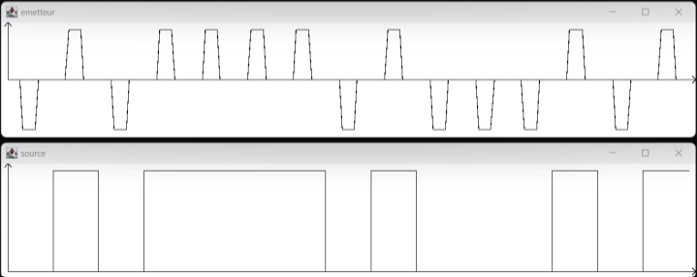
\includegraphics[width=1\textwidth]{image 11.png}
    \caption{\label{fig:image11}Sortie de la source et de l'émetteur RZ.}
\end{figure}

Ci-dessus le graphique en sortie de la source et de l'émetteur RZ. On apercevoir qu'un symbole logique est représenté par un symbole analogique composé en trois parties : le premier et dernier tiers à 0 et le deuxième tiers avec une amplitude à Vmax ou Vmin.

\textbf{Emetteur NRZT :}

C'est le transmetteur le plus complexe à faire. Il reprend les caractéristiques du NRZ mais possède une pente montante et descendante au 1er et dernier tiers. Avant toute chose, il faut calculer un pas qui sera utilisé pour la pente. Pour cela, on utilise cette formule : $ pas = \frac{Vx}{\frac{nb\_samples}{3}} $ avec Vx ayant Vmax ou Vmin en fonction du bit logique.

La construction d'un sylmbole se passe en trois étapes :
\begin{itemize}
    \item Sur le premier tiers $ \left(\frac{nb\_samples}{3} \right) $, les flottants ont une amplitude déterminée par le pas pour construire une rampe vers Vx.
    \item Sur le deuxième tiers $(]\frac{nb\_samples}{3}, \frac{nb\_samples}{3}*2]) $, les flottants ont pour valeur Vmax si le bit d'état logique est à 1 et Vmin si le bit est à 0.
    \item •	Sur le dernier tiers, les flottants ont une amplitude déterminée par le pas pour construire une rampe vers 0. Néanmoins, si plusieurs bits logiques de même signe se suivent, il n'y a pas de rampe entre le premier et le dernier tiers des bits analogiques correspondants. On reste sur une amplitude Vmax et Vmin.
\end{itemize}

\begin{figure}[h]
    \centering
    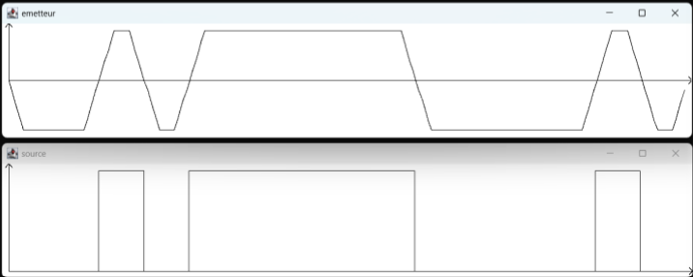
\includegraphics[width=1\textwidth]{image 12.png}
    \caption{\label{fig:image12}Sortie de la source et de l'émetteur NRZT.}
\end{figure}

Ci-dessus le graphique en sortie de la source et de l'émetteur NRZT. On remarque que le signal en sortie d'émetteur correspond bien à la description faite précédemment. On observe bien les pentes vers Vx et 0 mais également la conservation de l'amplitude Vx lorsque plusieurs bits logiques se suivent.

\subsubsection{Récepteur}

Le récepteur à un enjeu primordial, il est capable de recevoir un signal analogique et de le convertir en un signal logique (même type que le signal source). Notre exigence était d'avoir un seul récepteur qui puisse traiter n'importe quel signal analogique.
Pour ce faire, on utilise comme méthode de moyenner les valeurs reçues sur la durée d'un temps symbole. Préalablement, nous avons déterminer un seuil de décision qui correspond à $\frac{Vmax + Vmin}{2}$.
Il peut ainsi fluctuer en fonction des valeurs seuil choisi. Si la moyenne se situe au-dessus du seuil de décision, alors le bit d'état logique sera à 1. Si la moyenne se situe en-dessous du seuil de décision, alors le bit d'état logique sera à 0.

\subsection{Tests}

Par manque de temps, nous n'avons pas réalisé de test à proprement parler pour tester chaque ligne des nouvelles classes de l'itération. Nous avons seulement effectué un contrôle visuel grâce aux sondes placées aux différents endroits. Le principal contrôle étant de s'assurer que le signal reçu est le même que le signal émis comme il s'agit d'un canal parfait.
Pour les prochaines itérations, nous effectuerons de vrai test avec notamment des outils pour tester la couverture de ceux-ci.

\subsection{Performances}

Nous sommes toujours dans le cas d'un canal de transmission parfait. Que ce soit avec n'importe quel codage de signal, nous arrivons à retrouver les bits émis par la source.

Voici la simulation pour un signal généré grâce à une source aléatoire puis encodé en NRZ :

\begin{figure}[h]
    \centering
    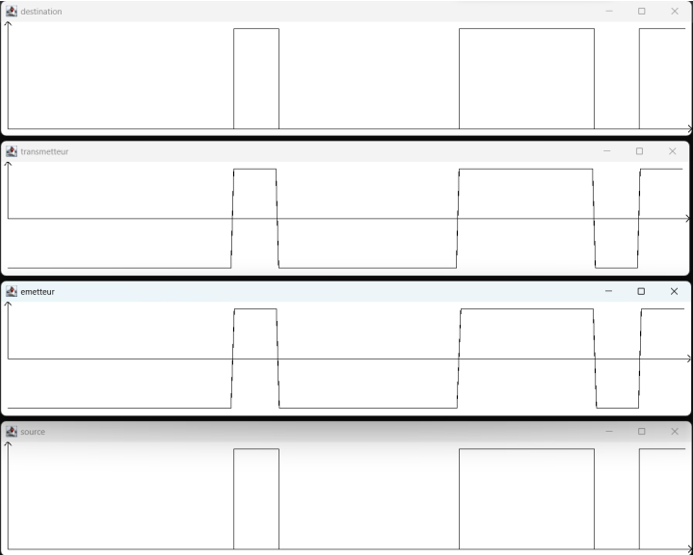
\includegraphics[width=1\textwidth]{image 13.png}
    \caption{\label{fig:image13}Simulation d'un signal généré puis encodé en NRZ.}
\end{figure}

Voici la simulation pour un signal généré grâce à une source aléatoire puis encodé en RZ :

\begin{figure}[h]
    \centering
    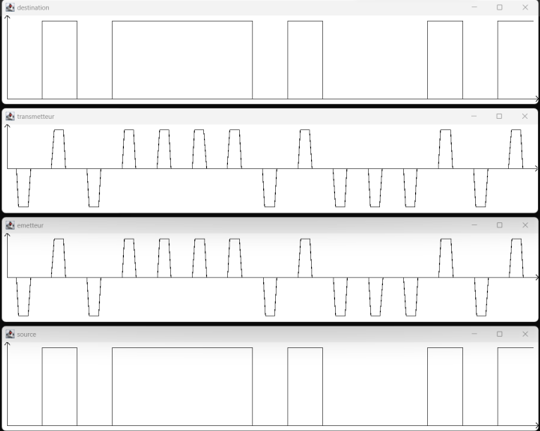
\includegraphics[width=1\textwidth]{image 14.png}
    \caption{\label{fig:image14}Simulation d'un signal généré puis encodé en RZ.}
\end{figure}

Voici la simulation pour un signal généré grâce à une source aléatoire puis encodé en NRZT :

\begin{figure}[h]
    \centering
    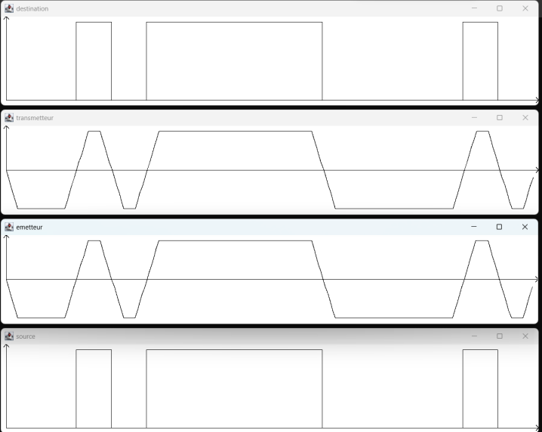
\includegraphics[width=1\textwidth]{image 15.png}
    \caption{\label{fig:image15}Simulation d'un signal généré puis encodé en NRZT.}
\end{figure}

Nous observons que la sortie du transmetteur est purement identique à la source. C'est normal car il s'agit d'un canal parfait. Le TEB est donc de 0. Le codage en ligne, quel qui soit, n'a pas d'impact
lorsqu'il est émis sur un transmetteur parfait.

\subsection{Conclusion}

Notre projet évolue. Lors de la première itération, notre chaine de transmission était opérationnelle avec comme fonctionnalités le type de source et l'observation de la sortie du canal.
Maintenant, nous sommes capables de convertir le signal de la source en un codage en ligne (RZ,NRZ et NRZT) et d'effectuer la manœuvre inverse en bout de canal afin de retrouver le signal de départ.

Nous avons également eu un problème de gestion du temps (mauvaise compréhension de la date de dépôt). Cette erreur ne nous a pas permis de livrer l'itération avec l'ensemble des attentes (tests, scripts). Ce manque sera comble lors de la prochaine itération.

Lors de la prochaine étape, il faudra créer un nouveau transmetteur afin d'avoir une transmission non-idéale avec canal bruité de type " gaussien ".

\pagebreak
\newpage

\section{Itération n°3}

\subsection{Objectif de l'itération}

Dans cette nouvelle itération, nous allons devoir modifier notre code afin que ce dernier puisse gérer les problèmes au niveau du bruit et de sa puissance. Nous allons devoir coder une nouvelle classe afin qu'elle émette un bruit gaussien. Par ailleurs, nous devrons mettre en place un code nous permettant d'échantiller les signaux bruités reçu afin qu'ils correspondent aux signaux émis.

Ci-dessous le schéma correspondant à l'itération n°3.

\begin{figure}[h]
    \centering
    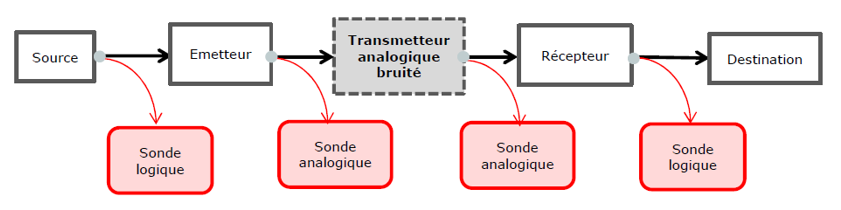
\includegraphics[width=1\textwidth]{image 16.png}
    \caption{\label{fig:image16}Schéma de l'itération n°3.}
\end{figure}

Ci-dessous le schéma correspondant à l'ajout de bruit pour cette itération

\begin{figure}[h]
    \centering
    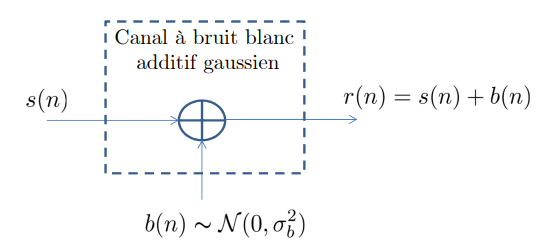
\includegraphics[width=0.8\textwidth]{image 17.png}
    \caption{\label{fig:image17}Schéma d'ajout de bruit itération n°3.}
\end{figure}


\subsection{Organisation}

\subsection{Procédures de développement}

\subsection{Tests}

\subsection{Performances}

\subsection{Conclusion}